\documentclass[a4paper,10pt]{article}
\usepackage[utf8]{inputenc}

\usepackage{graphicx}
\usepackage{float}
\usepackage{hyperref}

% Packages to embbed Matlab code
\usepackage[framed,numbered,autolinebreaks,useliterate]{mcode}
\usepackage{url,textcomp}
\setlength{\parindent}{0pt}

%opening
\title{Homework 2 - Robot Dynamics and Control}
\author{Erivelton Gualter dos Santos}

\begin{document}

\date{}
\maketitle

\section*{Preliminary steps}

\begin{enumerate}
 \item Determine the slight difference between Matlab’s \textit{atan2} and the function shown in Appendix A of SHV.
\end{enumerate}

The only difference between \textit{atan2} in SHV book and Matlab library is the order of the parameters. In Matlab, the y-axis parameter goes first, while the SHV book is opposite. For instance:

\begin{lstlisting}
    th = atan2(X,Y) % SHV notation
    th = atan2(Y,X) % Matlab notation
\end{lstlisting}


% Problem 1
\section{Problem}

Find the Euler angles equivalent to the following sequence ofrotations: Rotx($\frac{\pi}{2}$), Roty($-\pi$) (relative to $y_0$), Roty($\frac{\pi}{2}$) (relative to the current frame) and Rotz(-$\frac{\pi}{2}$) (relative toz0). Sketch all frames and verify that the Euler angles for the composite rotation work (if there are multiple solutions, show them all).

\hfill \break

The following figure illustrate the rotation by step-by-step:

\begin{figure}[H] 
 \centering
 \includegraphics[width=0.7\linewidth]{pb1.jpeg}
 \caption{Snapshot of frames.}\label{fig:frames}
\end{figure}

It is clearly that the last frame correspond to:

$$\left(\begin{array}{c} x'\\ y'\\ z' \end{array}\right)  = \left(\begin{array}{ccc} 1 & 0 & 0\\ 0 & 0 & 1\\ 0 & -1 & 0 \end{array}\right)\left(\begin{array}{c} x\\ y\\ z \end{array}\right) = \left(\begin{array}{c} x\\ z\\ -y \end{array}\right)$$

\begin{lstlisting}
%% Problem 1
R04 = Rotz(-sym(pi/2))*Roty(-sym(pi))*Rotx(sym(pi)/2)*Roty(sym(pi/2))

function out = Rotx(alpha)
%Rot_x: Basic rotation matrix about the x-axes 
out = [1 0 0 ; ...
    0 cos(alpha) -sin(alpha); ....
    0 sin(alpha) cos(alpha)]; 
end

function out = Roty(alpha)
%Rot_y: Basic rotation matrix about the y-axes 
out = [cos(alpha) 0 sin(alpha); ...
    0 1 0; ...
    -sin(alpha) 0 cos(alpha)]; 
end

function out = Rotz(alpha)
%Rot_z: Basic rotation matrix about the z-axes 
out = [cos(alpha) -sin(alpha) 0; ...
    sin(alpha) cos(alpha) 0; ...
    0 0 1]; 
end


\end{lstlisting}

\newpage

% Problem 2
\section{Problem}

Consider the PP robot with spherical wrist shown in Fig. \ref{fig:5dof}. Consider all 3 DOF of the spherical wrist to be concentric (zero lengths between joints)


\begin{figure}[H] 
 \centering
 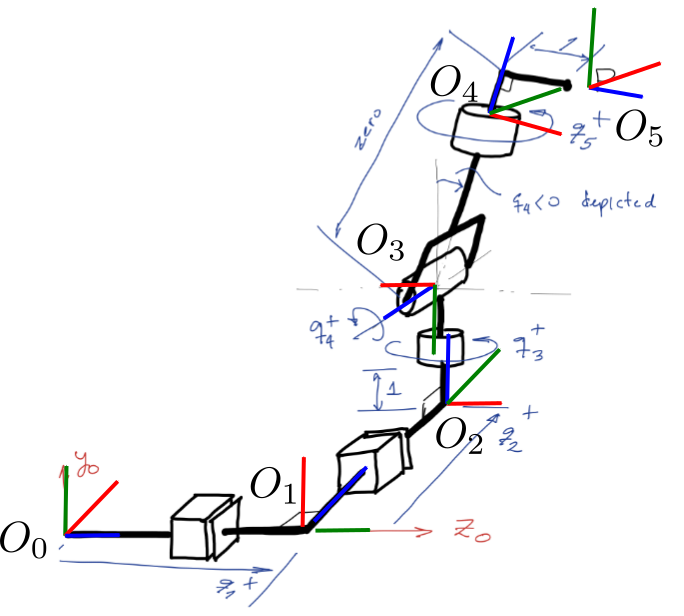
\includegraphics[width=0.7\linewidth]{5DOF.png}
 \caption{5-DOF robot with spherical wrist.}\label{fig:5dof}
\end{figure}


% Please add the following required packages to your document preamble:
% \usepackage{booktabs}
\begin{table}[H]
\caption{DH parameters for the 5-DOF manipulator.}
\begin{center}
\label{table:DH}
\begin{tabular}{c c c c c} \hline
Link & $a_i$ & $\alpha_i$       & $d_i$ & $\theta_i$      \\ \hline \hline
1    & 0     & $\frac{\pi}{2}$  & $q_1$ & $\frac{\pi}{2}$ \\
2    & 0     & $\frac{\pi}{2}$  & $q_2$ & $\frac{\pi}{2}$ \\
3    & 0     & $\frac{\pi}{2}$  & $q_3$ & $q_3$           \\
4    & 0     & $\frac{-\pi}{2}$ & 0     & $q_4$           \\
$^a$     & $d_5$ & 0                & 0     & $q_5$           \\
5    & 0     & $\frac{\pi}{2}$  & 0     & $\frac{\pi}{2}$ \\ \hline
\end{tabular}
\end{center}
\centering
\footnotesize{$^a$ Intermediate frame.}\\
\end{table}

After label the joint axes and stablished the base frame (Figure~\ref{fig:5dof}), a table of DH parameters were created (Table \ref{table:DH}). A configure for zero angle configuration is displayed in the Figure \ref{fig:conf0}. Additionally, two other ``easy'' configurations are illustrated at Figures \ref{fig:conf1} and \ref{fig:conf2}.
For a given joint coordinate functions, three figures were obtained: Figure \ref{fig:effecTime} correspond to the position of enf-effector along the time, Figure \ref{fig:effec3D} represent the enf-effector position on space, Figure \ref{fig:butterflyplanes} illustrates the trajectory on a variety of planes.

\begin{figure}[H] 
 \centering
 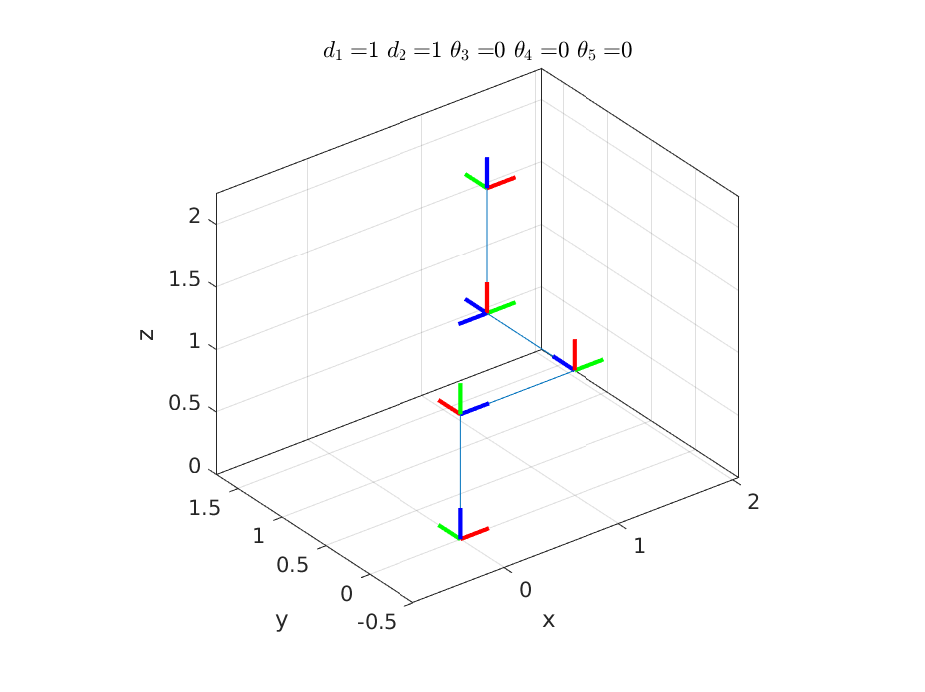
\includegraphics[width=1\linewidth]{configuration0.eps}
 \caption{Zero angle configuration.}\label{fig:conf0}
\end{figure}

\begin{figure}[H] 
 \centering
 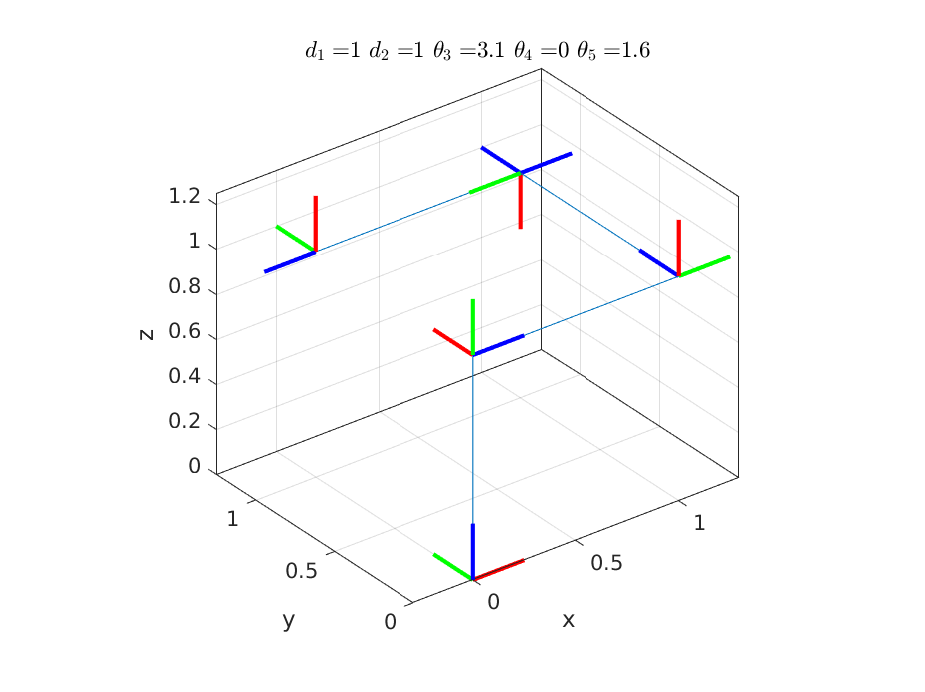
\includegraphics[width=1\linewidth]{configuration1.eps}
 \caption{``Easy'' configuration test \#1.}\label{fig:conf1}
\end{figure}

\begin{figure}[H] 
 \centering
 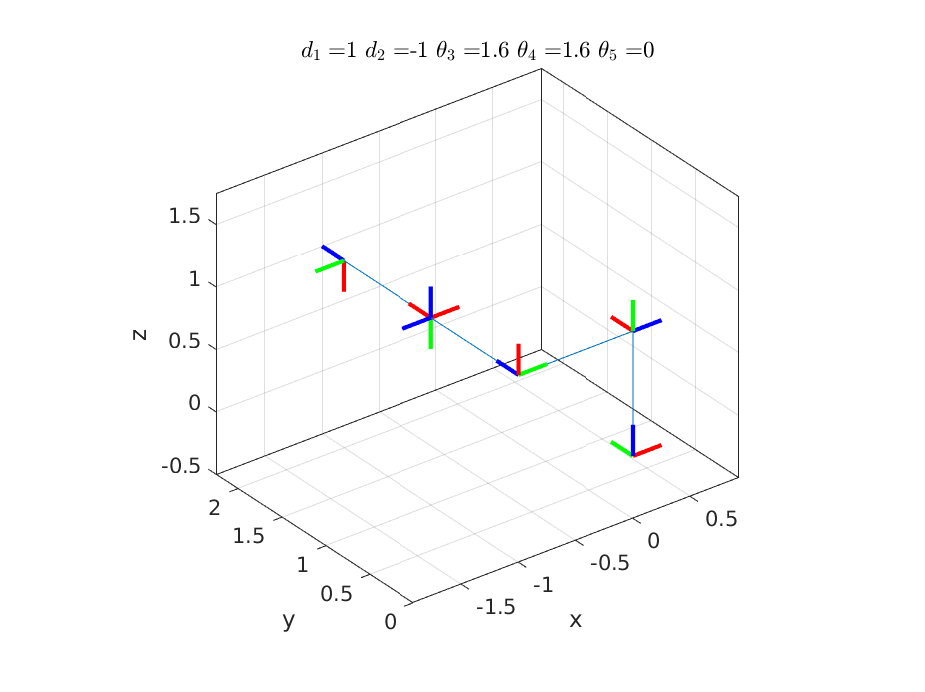
\includegraphics[width=1\linewidth]{configuration2.eps}\label{fig:conf2}
 \caption{``Easy'' configuration test \#2.}
\end{figure}

\begin{figure}[H] 
 \centering
 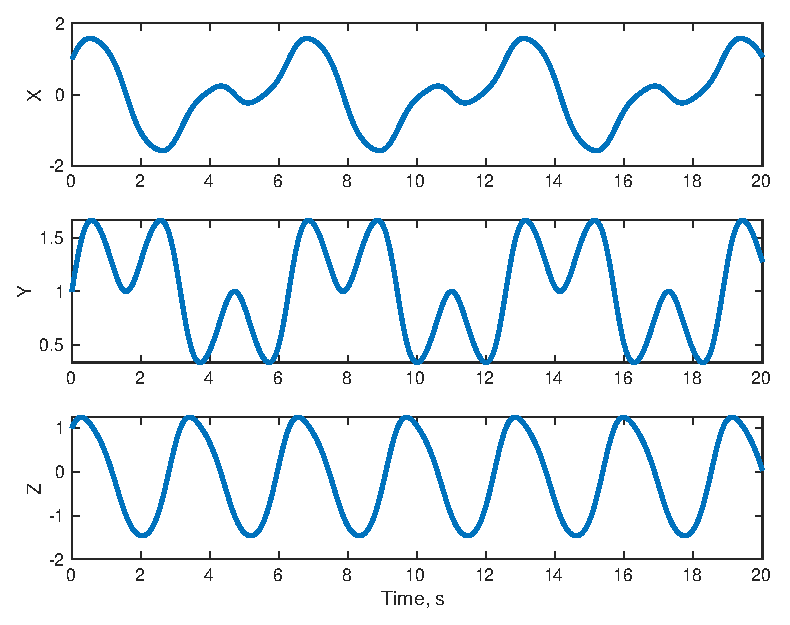
\includegraphics[width=.7\linewidth]{EndETrajTime.eps}
 \caption{Position of End-Effector along the time.}\label{fig:effecTime}
\end{figure}

\begin{figure}[H] 
 \centering
 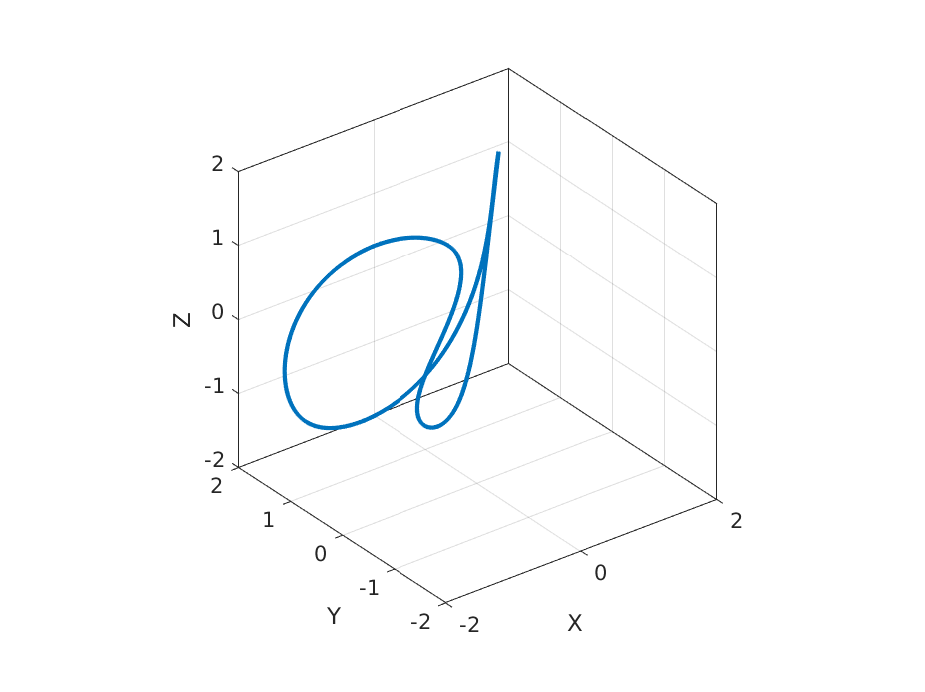
\includegraphics[width=1\linewidth]{EndETraj3D.eps}
 \caption{End-Effector trajectory on space.}\label{fig:effec3D}
\end{figure}

\begin{figure}[H] 
 \centering
 \includegraphics[width=1\linewidth]{butterflyplanes.eps}
 \caption{End-Effector trajectory on XY, YZ, and XZ planes.}\label{fig:butterflyplanes}
\end{figure}


% Problem 3
\section{Problem}

Consider the 4-axis SCARA robot shown in Fig. \ref{fig:ScaraFrame}. The spindle at the end of the second link can move vertically and also rotate through 360 degrees, providing two degrees of freedom that can be independently actuated. The robot will be used to cut a rectangular window on a circular-base cylinder. The cylinder has radius 50 mm, is 100 mm tall and is supporte 75 mm above the base of the robot. The cut should be completed in 20 seconds.

\hfill \break

\begin{figure}[H] 
 \centering
 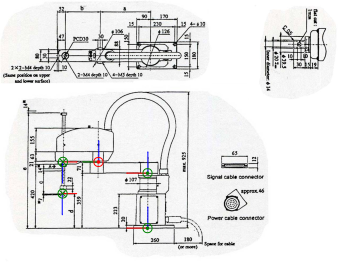
\includegraphics[width=0.7\linewidth]{SCARAview}
 \caption{Base frames}\label{fig:ScaraFrame}
\end{figure}

Figure \ref{fig:ScaraFrame} contains the established base frames in the robot. Following figure illustrated SCARA robot at zero angle configuration.

\begin{figure}[H] 
 \centering
 \includegraphics[width=.6\linewidth]{SCARAconf0}
 \caption{Plot of Robot at zero angle configuration.}\label{fig:ScaraConf0}
\end{figure}

The problem requires that the rectangular window to be cut at 20 seconds. In order to achieve that, it was found a average speed for the robot travel the total distance in 20 seconds. Then the trajectory path were found by $s=s_0+v\cdot t$, where $s$ is the position, $v$ is speed, and $t$ is the time.   

Figure ~\ref{fig:simulation} illustrates the simulation provided with this report. The top right zoom out in the cutting section, while in the bottow right shows the top view of the cutting. Note that the end-effector is tangent to the circle. 

\begin{figure}[H] 
 \centering
 \includegraphics[width=1\linewidth]{simulation.eps}
 \caption{Simulation Plot.}\label{fig:simulation}
\end{figure}

Following figure, correspond to the position from the direct and inverse kinematics \footnote{The derivations for the inverse kinematics equations in SHV is missing a power, the proof is attached to this report}. The RMS between them correspond to: $4.13\cdot10^{-14}$, $5.36\cdot10^{-14}$, and $1.87\cdot10^{-14}$.

\begin{figure}[H] 
 \centering
 \includegraphics[width=.8\linewidth]{INVvsDIR.eps}
 \caption{RMS for Inverse and Direct kinematics.}\label{fig:invdir}
\end{figure}

Additionally, the same problem was performed using the  Corke’s Robotics Toolbox. Following figure correspond to the robot at zero angle configuration. 

\begin{figure}[H] 
 \centering
 \includegraphics[width=1\linewidth]{toolboxZero}
 \caption{SCARA robot at zero angle configuration.}\label{toolbox}
\end{figure}

Following figure illustrates the position of end effector for the direct and inverse kinematic in order to evaluate the difference between them. The RMS error of them are: $4.54e-05$, $3.15e-04$, and $3.30e-08$. The error are still really small; however the analytical solution presented before were better than this one.

\begin{figure}[H] 
 \centering
 \includegraphics[width=.8\linewidth]{INVvsDIR3.eps}
 \caption{RMS for Inverse and Direct kinematics.}\label{fig:invdir2}
\end{figure}

\section{Code Instruction}

\begin{itemize}
 \item Download the ``HW2'', which contains the following code (\textbf{MAINroboticsHW2.m}) attached in the email. 
 \item Alternatively, the code is avaliable at \url{https://github.com/EriveltonGualter/MCE747-Robot-Dynamics-and-Control} after submission deadline.
 \item Due to the number of plots in this homework, you can run the code in parts. 
 \begin{itemize}
  \item Add ``Robotics Toolbox for Matlab (release 9.10)'' to the path.
  \item Problem 2: Run \textbf{MAINroboticsHW2(1)}.
  \item Problem 3 (SCARA robot): Run \textbf{MAINroboticsHW2(2)}.
  \item Problem 3 (SCARA robot using Corke's Robotics Toolbox): Run\textbf{MAINroboticsHW2(2)} \footnote{I faced a ``Java Error'' to run this code a couple times. You may face this as weel. Just try to run again.}.
  \end{itemize} 
\end{itemize}

\end{document}



